% IITG BSc (Hons) DS&AI Term Project Report — SIMPLE / CONDENSED VERSION
% A shorter, plainer-language companion to report.tex (the full report).
% Compile with pdfLaTeX on Overleaf. Upload with the three fig_*.png files.
\documentclass[a4paper,twocolumn,10pt]{article}

\usepackage[a4paper,top=2.2cm,bottom=2.2cm,left=1.9cm,right=1.9cm,columnsep=0.6cm]{geometry}
\usepackage{newtxtext,newtxmath}
\usepackage{amsmath,amssymb}
\usepackage{graphicx}
\usepackage{booktabs}
\usepackage{xurl}
\usepackage{titlesec}
\usepackage[labelfont=bf,labelsep=period,font=small]{caption}
\usepackage[hidelinks]{hyperref}

\titleformat{\section}{\centering\normalsize\bfseries}{\thesection.}{0.5em}{\MakeUppercase}
\titlespacing{\section}{0pt}{9pt}{5pt}
\renewcommand{\figurename}{Fig.}

\begin{document}

\twocolumn[{
\centering
{\large\bfseries FORECASTING DAILY EQUITY VOLATILITY: CAN MACHINE LEARNING BEAT CLASSICAL MODELS?\par}
\vspace{4mm}
{\itshape François Schmitt (Roll Number: 23035010523)\par}
\vspace{3mm}
Term Project Report (Short Version), Trimester 9\\
B.Sc.\ (Honours) Data Science and Artificial Intelligence\\
Indian Institute of Technology Guwahati, India\\
{\ttfamily f.schmitt@op.iitg.ac.in}\par
\vspace{6mm}
}]

\begin{center}\textbf{ABSTRACT}\end{center}
\noindent
This project asks a simple question: can machine-learning and deep-learning models forecast next-day stock-market volatility better than classical statistical models? Eight models were tested on 17 years of S\&P~500 daily returns using a strict walk-forward setup with no look-ahead bias. A plain GARCH(1,1) gave the best result on the main metric (QLIKE). XGBoost had the lowest RMSE and MAE, but no learned model beat the GARCH family where it matters. The project reproduces the well-known result that GARCH is very hard to beat on daily data.

\vspace{2mm}
\noindent\textbf{\textit{Index Terms:}} Volatility forecasting, GARCH, QLIKE, XGBoost, LSTM

\section{Introduction}
Volatility is the size of an asset's price swings. It matters for option pricing, risk limits and position sizing. The direction of tomorrow's return is essentially unpredictable, but its size is not: calm days follow calm days and wild days follow wild days. Classical models like GARCH have used this persistence for decades. This project checks whether modern machine-learning (XGBoost) and deep-learning (LSTM) models can do better, testing every model fairly inside one evaluation harness.

\section{Problem and Objectives}
The task is to forecast tomorrow's variance using only information available today. True volatility is never observed, so forecasts are scored against the squared return $r_t^2$, a noisy but unbiased proxy. The objectives were: (i) build honest classical baselines (naive, rolling, EWMA, and the GARCH family); (ii) build a leak-free walk-forward evaluation with RMSE, MAE, QLIKE and the Diebold–Mariano test; (iii) build a walk-forward XGBoost and a regularized LSTM; and (iv) compare all models and test whether any difference is statistically real.

\section{Method}
\textbf{Baselines.} Naive ($\hat\sigma_t^2=r_{t-1}^2$), 21-day rolling variance, and EWMA (RiskMetrics, $\lambda=0.94$).

\textbf{GARCH family.} GARCH(1,1) models variance as $\sigma_t^2=\omega+\alpha r_{t-1}^2+\beta\sigma_{t-1}^2$. GJR-GARCH and EGARCH add a leverage term so that falls raise volatility more than rises. Parameters are re-estimated about monthly and rolled forward daily.

\textbf{Learned models.} XGBoost and an LSTM use the same features (recent returns, squared returns, and 5- and 21-day realized variance) and the same target (log of a 5-day-forward smoothed variance). XGBoost is re-trained about monthly; the LSTM uses train-only scaling and early stopping. Both respect the walk-forward rule: no future data leaks into any forecast.

\textbf{Scoring.} QLIKE is the headline metric because its model ranking is robust to noise in the proxy and it punishes under-prediction of variance. The Diebold–Mariano test checks whether a gap in loss is real or luck.

\section{Experiments and Results}
\textbf{Data.} S\&P~500 daily closes (2008--2024, Yahoo Finance), 4{,}277 returns. The last 30\% (1{,}284 days, 2019-11-21 to 2024-12-30, including the COVID crash) is the out-of-sample test window shared by every model.

Table~\ref{tab:lb} shows the leaderboard. GARCH(1,1) wins on QLIKE. The three GARCH-family models are statistically tied: Diebold–Mariano for GARCH(1,1) versus EGARCH(1,1) gives $p=0.87$ (not significant). XGBoost has the best RMSE and MAE but ranks fifth on QLIKE, because its smoothed target makes it accurate on average yet slow to react at volatility spikes. Fig.~\ref{fig:best} shows the winning forecast tracking realized volatility.

\begin{table}[t]
\centering
\caption{Leaderboard over the test window, sorted by QLIKE (lower is better).}
\label{tab:lb}
\small
\begin{tabular}{lrrr}
\toprule
Model & RMSE & MAE & QLIKE \\
\midrule
GARCH(1,1)      & 0.00887 & 0.00633 & \textbf{1.4879} \\
EGARCH(1,1)     & 0.00852 & 0.00603 & 1.4943 \\
GJR-GARCH(1,1)  & 0.00881 & 0.00611 & 1.4974 \\
EWMA(0.94)      & 0.00934 & 0.00657 & 1.5161 \\
XGBoost         & \textbf{0.00816} & \textbf{0.00547} & 1.5567 \\
Rolling(21)     & 0.00948 & 0.00646 & 1.5798 \\
LSTM            & 0.00965 & 0.00570 & 1.5915 \\
Naive           & 0.01114 & 0.00747 & 1192.69 \\
\bottomrule
\end{tabular}
\end{table}

\begin{figure}[t]
\centering
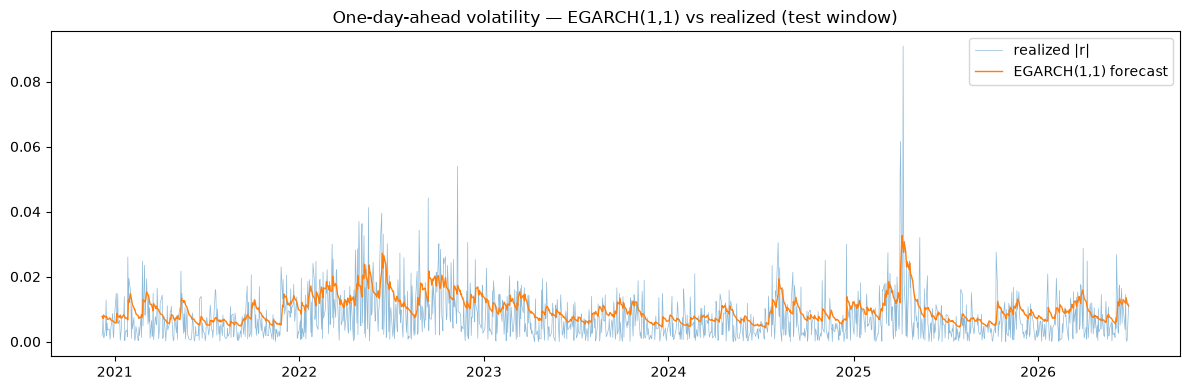
\includegraphics[width=\columnwidth]{fig_best_vs_realized.png}
\caption{Best model by QLIKE, GARCH(1,1), against realized volatility over the test window.}
\label{fig:best}
\end{figure}

\section{Discussion}
GARCH is hard to beat for four reasons. The signal is one-dimensional (persistence in return size), and GARCH is built exactly for it with only three parameters. GARCH is fit by maximum likelihood on the right objective, while the learned models train on a smoother substitute target. Daily data is small data, which favours simple models over neural networks. Finally, QLIKE rewards fast reactions to spikes, and GARCH reacts the next day. The main limitations are the single asset and test window, the noisy squared-return proxy, and modest hyperparameter tuning.

\section{Conclusion}
Under a leak-free walk-forward test on 17 years of S\&P~500 data, a monthly re-estimated GARCH(1,1) gave the best one-day-ahead volatility forecasts, and no learned model beat the GARCH family on QLIKE. The learned models were competitive but not better where it counts. The clearest lesson was methodological: a leak-free evaluation and the choice of metric matter more than model complexity. Useful next steps are intraday realized-variance targets, extra inputs such as the VIX, and multi-asset training.

\section{Artifacts}
Code: \url{https://github.com/iitgF/T9} (the \texttt{volforecast} package and notebooks). LaTeX source (Overleaf): \url{https://www.overleaf.com/project/6a48e18e7dee3049b3ee4209}. Full report: \texttt{report.tex}. AI-assisted tooling was used for refactoring and drafting; all decisions, checks and the final text are the author's, and every number was reproduced from the committed code.

\begin{thebibliography}{9}
\small
\bibitem{bollerslev1986}
T.~Bollerslev, ``Generalized autoregressive conditional heteroskedasticity,'' \textit{J. Econometrics}, vol.~31, no.~3, pp. 307--327, 1986. \url{https://doi.org/10.1016/0304-4076(86)90063-1}

\bibitem{glosten1993}
L.~R. Glosten, R.~Jagannathan, and D.~E. Runkle, ``On the relation between the expected value and the volatility of the nominal excess return on stocks,'' \textit{J. Finance}, vol.~48, no.~5, pp. 1779--1801, 1993. \url{https://doi.org/10.1111/j.1540-6261.1993.tb05128.x}

\bibitem{hansen2005}
P.~R. Hansen and A.~Lunde, ``A forecast comparison of volatility models: Does anything beat a GARCH(1,1)?'' \textit{J. Applied Econometrics}, vol.~20, no.~7, pp. 873--889, 2005. \url{https://doi.org/10.1002/jae.800}

\bibitem{patton2011}
A.~J. Patton, ``Volatility forecast comparison using imperfect volatility proxies,'' \textit{J. Econometrics}, vol.~160, no.~1, pp. 246--256, 2011. \url{https://doi.org/10.1016/j.jeconom.2010.03.034}
\end{thebibliography}

\end{document}
